\documentclass[11pt,compress,t,notes=noshow, xcolor=table]{beamer}
\usepackage[]{graphicx}\usepackage[]{color}
% maxwidth is the original width if it is less than linewidth
% otherwise use linewidth (to make sure the graphics do not exceed the margin)
\makeatletter
\def\maxwidth{ %
  \ifdim\Gin@nat@width>\linewidth
    \linewidth
  \else
    \Gin@nat@width
  \fi
}
\makeatother

\newcommand{\citebutton}[2]{%
\beamergotobutton{\href{#2}{#1}}%
}

\newcommand{\blu}[1]{\textcolor{blue}{#1}}
\newcommand{\org}[1]{\textcolor{orange}{#1}}
\newcommand{\ques}{\textbf{\textcolor{red}{Question:  }}}
\newcommand{\questionssofar}{\begin{frame}\frametitle{Any questions?}\end{frame}}

\newcommand\warning{%
 \makebox[1.4em][c]{%
 \makebox[0pt][c]{\raisebox{.1em}{\scriptsize!}}%
 \makebox[0pt][c]{\color{red}\normalsize$\bigtriangleup$}}}%

\definecolor{fgcolor}{rgb}{0.345, 0.345, 0.345}
\newcommand{\hlnum}[1]{\textcolor[rgb]{0.686,0.059,0.569}{#1}}%
\newcommand{\hlstr}[1]{\textcolor[rgb]{0.192,0.494,0.8}{#1}}%
\newcommand{\hlcom}[1]{\textcolor[rgb]{0.678,0.584,0.686}{\textit{#1}}}%
\newcommand{\hlopt}[1]{\textcolor[rgb]{0,0,0}{#1}}%
\newcommand{\hlstd}[1]{\textcolor[rgb]{0.345,0.345,0.345}{#1}}%
\newcommand{\hlkwa}[1]{\textcolor[rgb]{0.161,0.373,0.58}{\textbf{#1}}}%
\newcommand{\hlkwb}[1]{\textcolor[rgb]{0.69,0.353,0.396}{#1}}%
\newcommand{\hlkwc}[1]{\textcolor[rgb]{0.333,0.667,0.333}{#1}}%
\newcommand{\hlkwd}[1]{\textcolor[rgb]{0.737,0.353,0.396}{\textbf{#1}}}%
\let\hlipl\hlkwb

\usepackage{framed}
\makeatletter
\newenvironment{kframe}{%
 \def\at@end@of@kframe{}%
 \ifinner\ifhmode%
  \def\at@end@of@kframe{\end{minipage}}%
  \begin{minipage}{\columnwidth}%
 \fi\fi%
 \def\FrameCommand##1{\hskip\@totalleftmargin \hskip-\fboxsep
 \colorbox{shadecolor}{##1}\hskip-\fboxsep
     % There is no \\@totalrightmargin, so:
     \hskip-\linewidth \hskip-\@totalleftmargin \hskip\columnwidth}%
 \MakeFramed {\advance\hsize-\width
   \@totalleftmargin\z@ \linewidth\hsize
   \@setminipage}}%
 {\par\unskip\endMakeFramed%
 \at@end@of@kframe}
\makeatother

\definecolor{shadecolor}{rgb}{.97, .97, .97}
\definecolor{messagecolor}{rgb}{0, 0, 0}
\definecolor{warningcolor}{rgb}{1, 0, 1}
\definecolor{errorcolor}{rgb}{1, 0, 0}
\newenvironment{knitrout}{}{} % an empty environment to be redefined in TeX

\usepackage{alltt}
\newcommand{\SweaveOpts}[1]{}  % do not interfere with LaTeX
\newcommand{\SweaveInput}[1]{} % because they are not real TeX commands
\newcommand{\Sexpr}[1]{}       % will only be parsed by R
\newcommand{\xmark}{\ding{55}}%


\usepackage[english]{babel}
\usepackage[utf8]{inputenc}

\usepackage{dsfont}
\usepackage{verbatim}
\usepackage{amsmath}
\usepackage{amsfonts}
\usepackage{amssymb}
\usepackage{bm}
\usepackage{csquotes}
\usepackage{multirow}
\usepackage{longtable}
\usepackage{booktabs}
\usepackage{enumerate}
\usepackage[absolute,overlay]{textpos}
\usepackage{psfrag}
\usepackage{algorithm}
\usepackage{algpseudocode}
\usepackage{eqnarray}
\usepackage{arydshln}
\usepackage{tabularx}
\usepackage{placeins}
\usepackage{tikz}
\usepackage{setspace}
\usepackage{colortbl}
\usepackage{mathtools}
\usepackage{wrapfig}
\usepackage{bm}
\usepackage{amsmath}
\usepackage{pifont}

\usetikzlibrary{shapes.multipart,shapes,arrows,automata,positioning,calc,chains,trees, shadows}
\tikzset{
  %Define standard arrow tip
  >=stealth',
  %Define style for boxes
  punkt/.style={
    rectangle,
    rounded corners,
    draw=black, very thick,
    text width=6.5em,
    minimum height=2em,
    text centered},
  % Define arrow style
  pil/.style={
    ->,
    thick,
    shorten <=2pt,
    shorten >=2pt,}
}

\tikzstyle{vec}=[draw, rectangle, fill = white, minimum width=5mm, minimum height=1cm, inner sep = 2pt]

\usepackage{subfig}

% Defines macros and environments
\usepackage{../../style/lmu-lecture}


\let\code=\texttt
\let\proglang=\textsf

\setkeys{Gin}{width=0.9\textwidth}

\setbeamertemplate{frametitle}{\expandafter\uppercase\expandafter\insertframetitle}

\usepackage{bbm}
% basic latex stuff
\newcommand{\pkg}[1]{{\fontseries{b}\selectfont #1}} %fontstyle for R packages
\newcommand{\lz}{\vspace{0.5cm}} %vertical space
\newcommand{\dlz}{\vspace{1cm}} %double vertical space
\newcommand{\oneliner}[1] % Oneliner for important statements
{\begin{block}{}\begin{center}\begin{Large}#1\end{Large}\end{center}\end{block}}


%new environments
\newenvironment{vbframe}  %frame with breaks and verbatim
{
 \begin{frame}[containsverbatim,allowframebreaks]
}
{
\end{frame}
}

\newenvironment{vframe}  %frame with verbatim without breaks (to avoid numbering one slided frames)
{
 \begin{frame}[containsverbatim]
}
{
\end{frame}
}

\newenvironment{blocki}[1]   % itemize block
{
 \begin{block}{#1}\begin{itemize}
}
{
\end{itemize}\end{block}
}

\newenvironment{fragileframe}[2]{  %fragile frame with framebreaks
\begin{frame}[allowframebreaks, fragile, environment = fragileframe]
\frametitle{#1}
#2}
{\end{frame}}


\newcommand{\myframe}[2]{  %short for frame with framebreaks
\begin{frame}[allowframebreaks]
\frametitle{#1}
#2
\end{frame}}

\newcommand{\remark}[1]{
  \textbf{Remark:} #1
}


\newenvironment{deleteframe}
{
\begingroup
\usebackgroundtemplate{
\includegraphics[width=\paperwidth,height=\paperheight]{../style/color/red.png}}
 \begin{frame}
}
{
\end{frame}
\endgroup
}
\newenvironment{simplifyframe}
{
\begingroup
\usebackgroundtemplate{
\includegraphics[width=\paperwidth,height=\paperheight]{../style/color/yellow.png}}
 \begin{frame}
}
{
\end{frame}
\endgroup
}\newenvironment{draftframe}
{
\begingroup
\usebackgroundtemplate{
\includegraphics[width=\paperwidth,height=\paperheight]{../style/color/green.jpg}}
 \begin{frame}
}
{
\end{frame}
\endgroup
}
% https://tex.stackexchange.com/a/261480: textcolor that works in mathmode
\makeatletter
\renewcommand*{\@textcolor}[3]{%
  \protect\leavevmode
  \begingroup
    \color#1{#2}#3%
  \endgroup
}
\makeatother





\input{../../latex-math/basic-math.tex}
\input{../../latex-math/basic-ml.tex}

%\newcommand{\titlefigure}{figure/gpt_sq.png}
\newcommand{\learninggoals}{
\item comprehend the different subtleties in the space of fine-tuning and prompting}

\definecolor{texblue}{rgb}{0, 0, 1}
\def\myblue#1{\textcolor{texblue}{#1}}

\title{Large Language Models (LLMs)}
% \author{}
\institute{\href{https://slds-lmu.github.io/lecture_dl4nlp/}{slds-lmu.github.io/lecture\_dl4nlp}}
\date{}

\begin{document}
\lecturechapter{Fine-Tuning}
\lecture{Deep Learning for NLP}

% ------------------------------------------------------------------------------

\begin{frame}{recap}

\vfill

\begin{itemize}
    \item language modeling objectives
        \begin{itemize}
            \item token prediction
            \item no explicit understanding of tasks
        \end{itemize}
    \item this is true for encoder and decoder models
    \item So we need to do additional work if we want
        to use language models for solving tasks!
\end{itemize}

\vfill

\end{frame}


\begin{frame}{How to solve a task with language models? (1)}

\vfill

\begin{itemize}
    \item ``old-style'' single-task fine-tuning 
        \begin{itemize}
            \item supervised training on a task-specific
        training set of size $k$ (where $k$ is not small,
        e.g., $k=100$)
        \end{itemize}
\end{itemize}

\vfill

\end{frame}

\begin{frame}{BERT finetuning example 1}

\vfill
	
	\begin{figure}
		\centering
		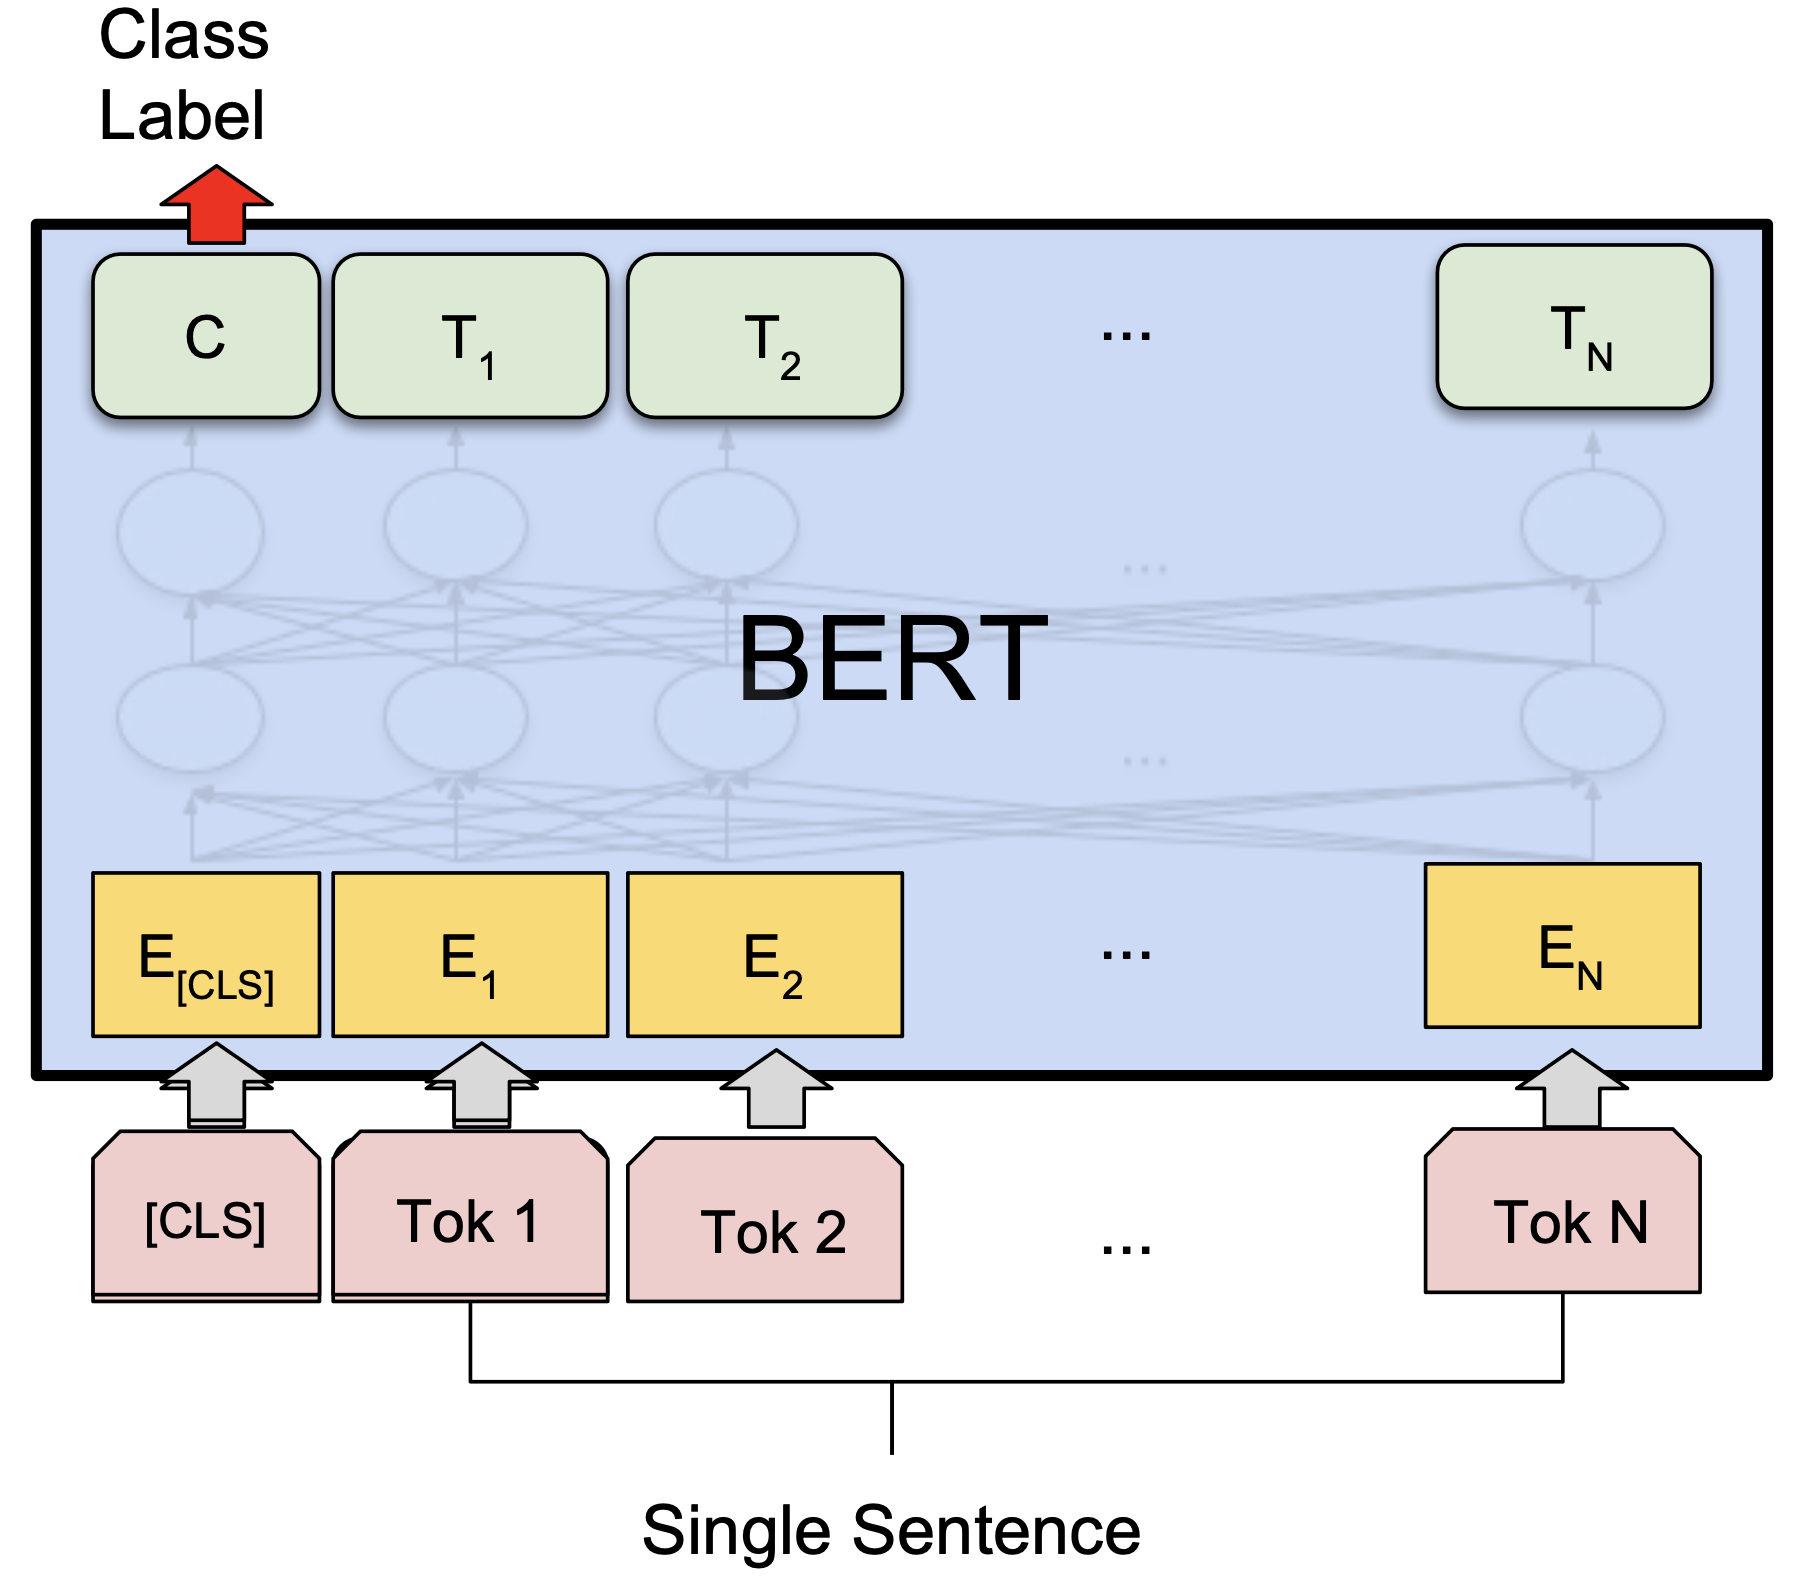
\includegraphics[height = 6cm]{figure/bertfinetune1} 
	\end{figure}

\vfill

\end{frame}
\begin{frame}{BERT finetuning example 2}

\vfill
	
	\begin{figure}
		\centering
		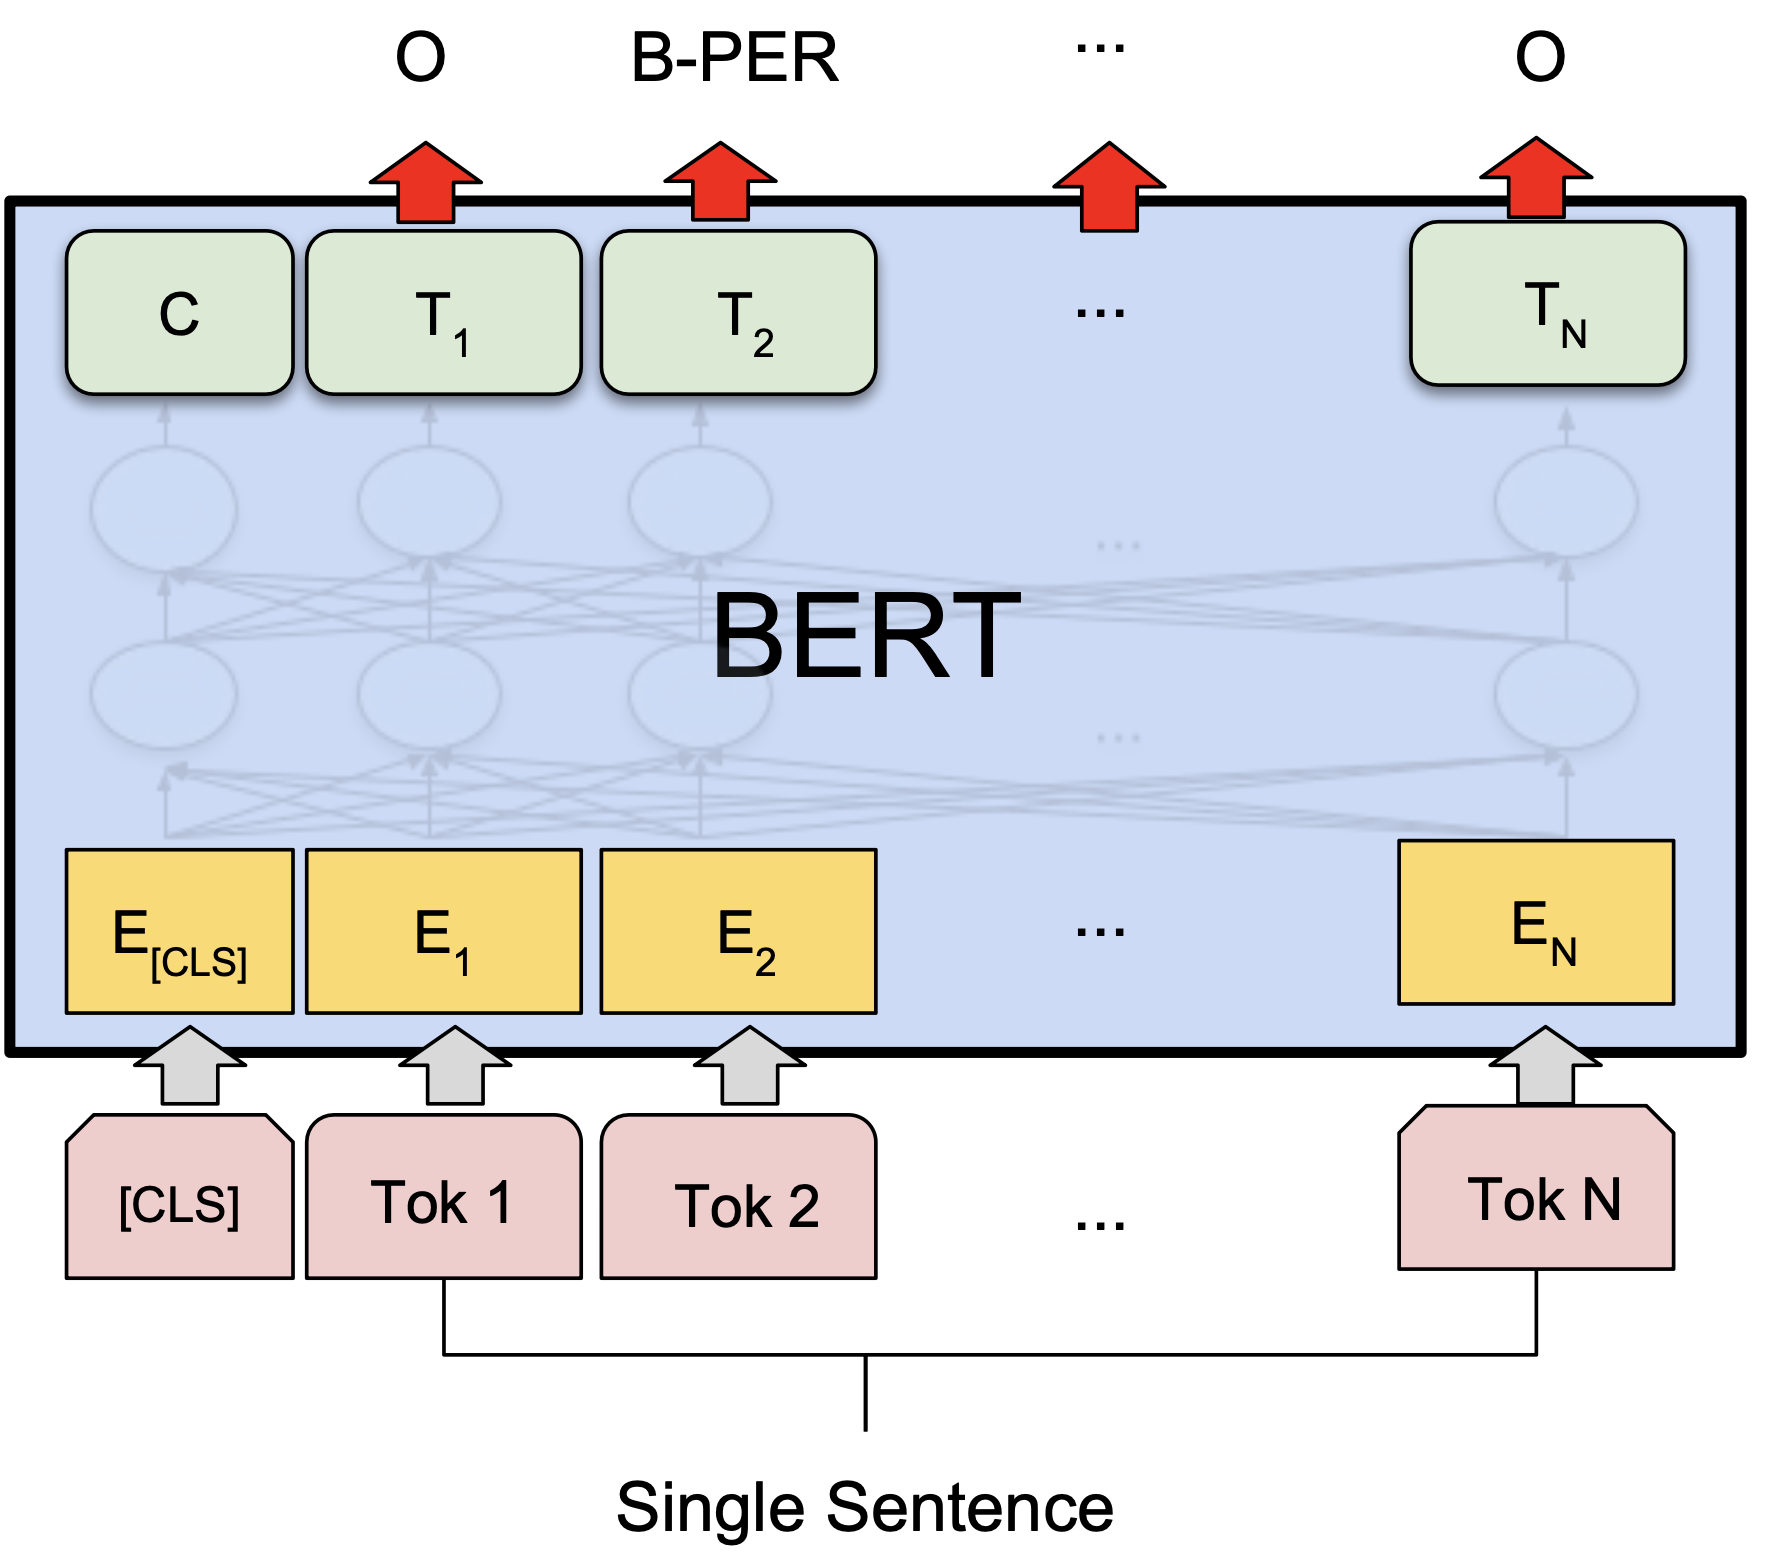
\includegraphics[height = 6cm]{figure/bertfinetune2} 
	\end{figure}

\vfill

\end{frame}


\begin{frame}{How to solve a task with language models? (1)}

\vfill

\begin{itemize}
    \item ``old-style'' single-task fine-tuning 
        \begin{itemize}
            \item supervised training on a task-specific
        training set of size $k$ (where $k$ is not small,
        e.g., $k=100$)
        \item the output can be an arbitrary category (e.g.,
        ``0'', ``1'' for sentiment analysis)
            \item alternatively, the output can be a
        meaningful ``verbalizer'' (e.g., ``negative'',
        ``positive'' for sentiment analysis)
        		\citebutton{Schick et al.,
        2020}{https://arxiv.org/abs/2009.07118}
        \item this was the typical way encoder models like
        BERT are used
        \item still very much relevant if you need to deploy
        a small efficient model for a focused task
\item draw picture
        \end{itemize}
\end{itemize}

\vfill

\end{frame}












\begin{frame}{How to solve a task with language models? (2)}

\vfill

\begin{itemize}
    \item few-shot prompting
        \begin{itemize}
            \item provide, in-context,  $k$ (where $k$ is small, e.g., $k=5$) examples of what the model is
supposed to do
        \item the model will then often complete the task
        just based on analogy to these few shots
        \item this is the most typical way of using current
        autoregressive models for tasks
\item no change to the parameters of the model, i.e., no training
\end{itemize}
\end{itemize}

\vfill

\end{frame}

\begin{frame}{few-shot prompting example}

\vfill
	
	\begin{figure}
		\centering
		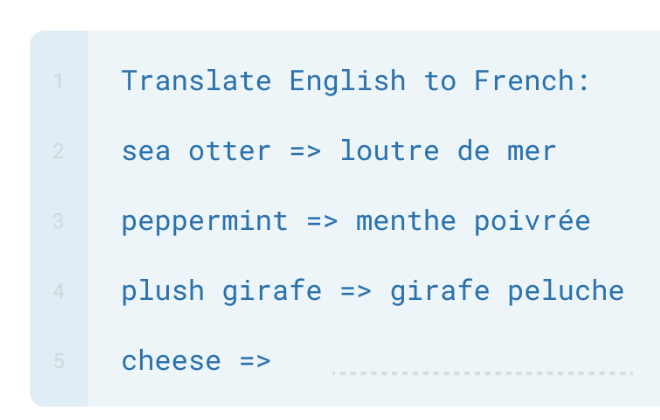
\includegraphics[height = 6cm]{figure/fewshotprompting} 
	\end{figure}

\vfill

\end{frame}


\begin{frame}{How to solve a task with language models? (3)}

\vfill

\begin{itemize}
\item multi-task finetuning
        \begin{itemize}
        \item finetuning on a large training set of *many* tasks
        \item the more tasks the better
        \item method 1: consistent task format, e.g., each
        task is reformulated into a question-answering format
        \item method 2: more open task format
\item ideally: task format is
consistent with language model
            objective (similar to verbalizer)
            \item Examples: T5 and FLAN, see below
        \end{itemize}
\end{itemize}

\vfill

\end{frame}

\begin{frame}{How to solve a task with language models? (4)}

\vfill

\begin{itemize}
\item instruction tuning (short for instruction finetuning)
        \begin{itemize}
            \item you teach the model a *general*
            capability of being ``helpful''
            \item it then solves arbitrary tasks without few-shot
            prompting and without additional finetuning
            \item theory/hope: you no longer have to explicitly
            train on specific tasks, the instruction-tuned
            model can solve new tasks without having been
            trained on them
            \item next lecture
        \end{itemize}
\end{itemize}

\vfill

\end{frame}

% ------------------------------------------------------------------------------

% ------------------------------------------------------------------------------

\begin{frame}{Another type of finetuning}

\vfill

\begin{itemize}
    \item Finetuning has yet another meaning.
    \item Continued pretraining is also sometimes called
    finetuning.
    \item Continued pretraining: given a language model
that has been    trained on generic data (web, reddit etc),
    adapt it to a new domain (e.g., company-internal data) by
    training it on a large corpus from this new domain.
\item objective: standard language modeling objective
    \item This results in a language model that has all the
    nice capabilities of a generic language model (e.g.,
    MISTRAL family), but also understands the special domain.
\item Not trivial to do well
\end{itemize}

\vfill

\end{frame}

\begin{frame}{Finetuning: Terminology}

\vfill

\begin{itemize}
\item single-task finetuning
\item multi-task finetuning
\item instruction tuning\\ (can be seen as a form of finetuning)
\item prompting\\
(this is definitely not finetuning)
\item continued pretraining
\item \ques terminology clear?
\end{itemize}

\vfill

\end{frame}


% ------------------------------------------------------------------------------


% ------------------------------------------------------------------------------

%\begin{frame}{pre-trained generative models}
%
%\vfill
%	
%	\begin{figure}
%		\centering
%		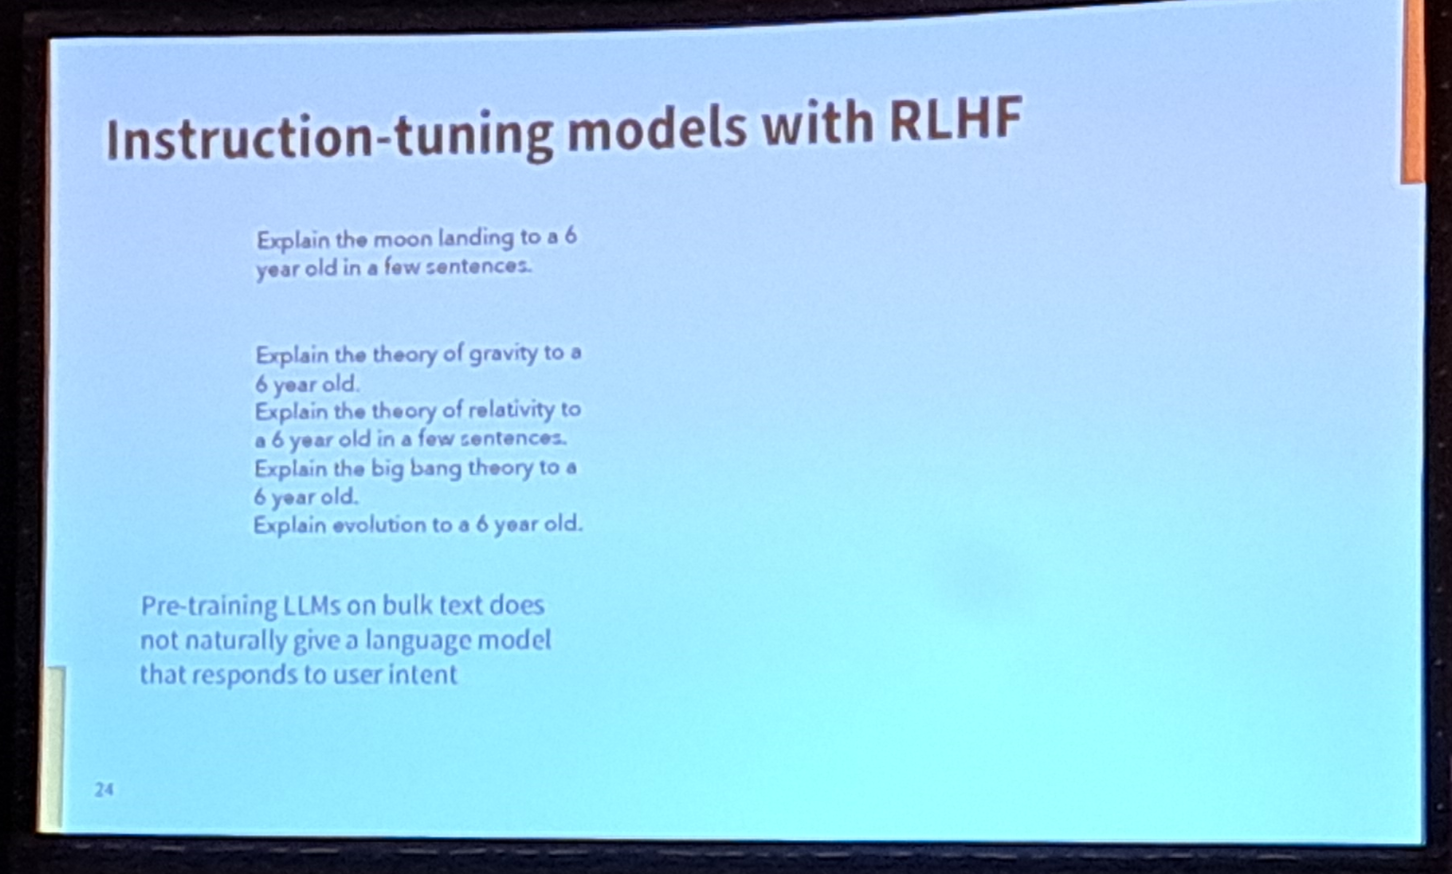
\includegraphics[width = 11cm]{figure/manning.png}\\ 
%		Source: Chris Manning's keynote at EMNLP 2023
%	\end{figure}
%
%\vfill
%
%\end{frame}

% ------------------------------------------------------------------------------

%\begin{frame}{agenda}
%
%\vfill
%
%\begin{itemize}
%    \item \textit{chain-of-thought prompting:}
%        \begin{itemize}
%            \item trigger the model to ''explain'' it thought-process
%            \item final goal still correct label/output
%        \end{itemize}
%    \item \textit{emergent abilities:}
%        \begin{itemize}
%%%%%%%%            \item \textit{claim:} With increasing model sizes, at some point new capabilities of the models (seem to) ''emerge''.
%        \end{itemize}
%\end{itemize}
%
%\vfill
%
%\end{frame}

% ------------------------------------------------------------------------------

\begin{frame}{issues with single-task fine-tuning}

\vfill

\begin{itemize}
    \item The result is a single-task model.
\item Sequential transfer learning instead of multi-task learning
    \item Generalization of the model 
             only w.r.t. to one task / data distribution
    \item Requires quite a bit of annotated
        data (e.g., $k=100$)
    \item Single-task models have poor few-shot capabilities
            \item \ques Could there be other tasks that
        might benefit?
            \item \ques What about related domains / languages?
\end{itemize}

\vfill

\end{frame}

% ------------------------------------------------------------------------------
\begin{frame}{issues with prompting}

\vfill

\begin{itemize}
    \item Assumption: Model has learned about the task during (unsupervised) pre-training 
    \item Write prompt so that  a direct response must be
    given by the language model.
        \item Just a label, just yes/no answer, just a name
    in QA
    \item This is not natural dialogic behavior: humans
    typically don't
    just answer with a label, yes/no, a name (although
    sometimes they do)
    \item See next lecture
\item Again: Prompting works best if the task has occurred during
unsupervised training.
    \item \ques For which tasks is this expected to work well?
% machine translation example:  example of what works well
% complex reasoning example: example of what does notw ork well
%    \item \textit{Lack of interpretability}
%    \begin{itemize}
%        \item Just the answer w/o explanation
%        \item Big concern about LLMs in general

%    \item \textit{Misalignment with human needs}
%    \begin{itemize}
%        \item Out of context answers
%        \item Harmful answers
%    \end{itemize}
\end{itemize}

\vfill

\end{frame}
% ------------------------------------------------------------------------------

%\begin{vbframe}{issues with prompting}
%
%\vfill
%
%\begin{itemize}
%    \item \textit{Hallucinations:} Output that is not true.
%(different possible causes: just made up,
%incorrect internal reasoning etc)
%    \item \textit{Imprecise mathematical operations:} Models not trained to do arithmetics
%    \item \textit{Inadequate experience grounding:} Not
%    fully capable of generating correct answers to questions
%    from specialized domains not covered by pretraining data
%    \item \textit{Limited ability for complex reasoning:} Long-known challenge in NLP/LLMs
%\end{itemize}
%
%\vfill
%
%\end{vbframe}
%
%% ------------------------------------------------------------------------------

%\begin{frame}{issues with prompting}
%
%\vfill
%
%\begin{itemize}
%% if you believe that you can find everything on the web: yes
%% however: see point "grounding in specialized domain" in a few slides
%    \end{itemize}
%
%
%\vfill
%
%\end{frame}


\begin{frame}{Multitask finetuning: best of both worlds
(finetuning and  prompting)}

\vfill
	
	\begin{figure}
		\centering
		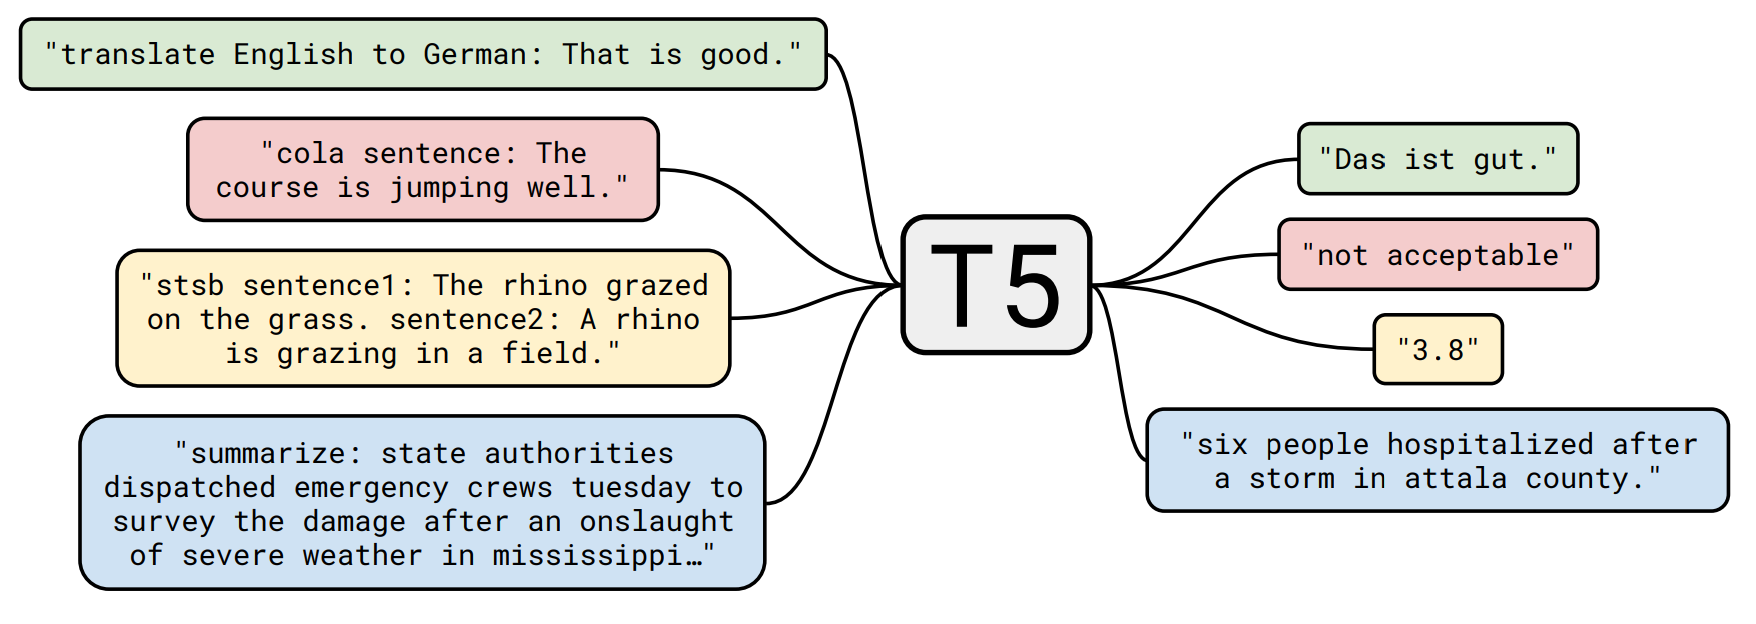
\includegraphics[width = 11cm]{figure/62-t5.png}\\ 
		\citebutton{Source: Raffel et al., 2020}{https://jmlr.org/papers/v21/20-074.html}
	\end{figure}

\pause

     \ques What exactly does the model learn here? How well
    would we expect this to generalize to new tasks?
    % IMPLICITLY, i.e. the model learns via fine-tuning which task prefix to associate with which set of labels


\vfill

\end{frame}

% ------------------------------------------------------------------------------


\begin{frame}{Construction of training set}

\vfill
	
	\begin{figure}
		\centering
		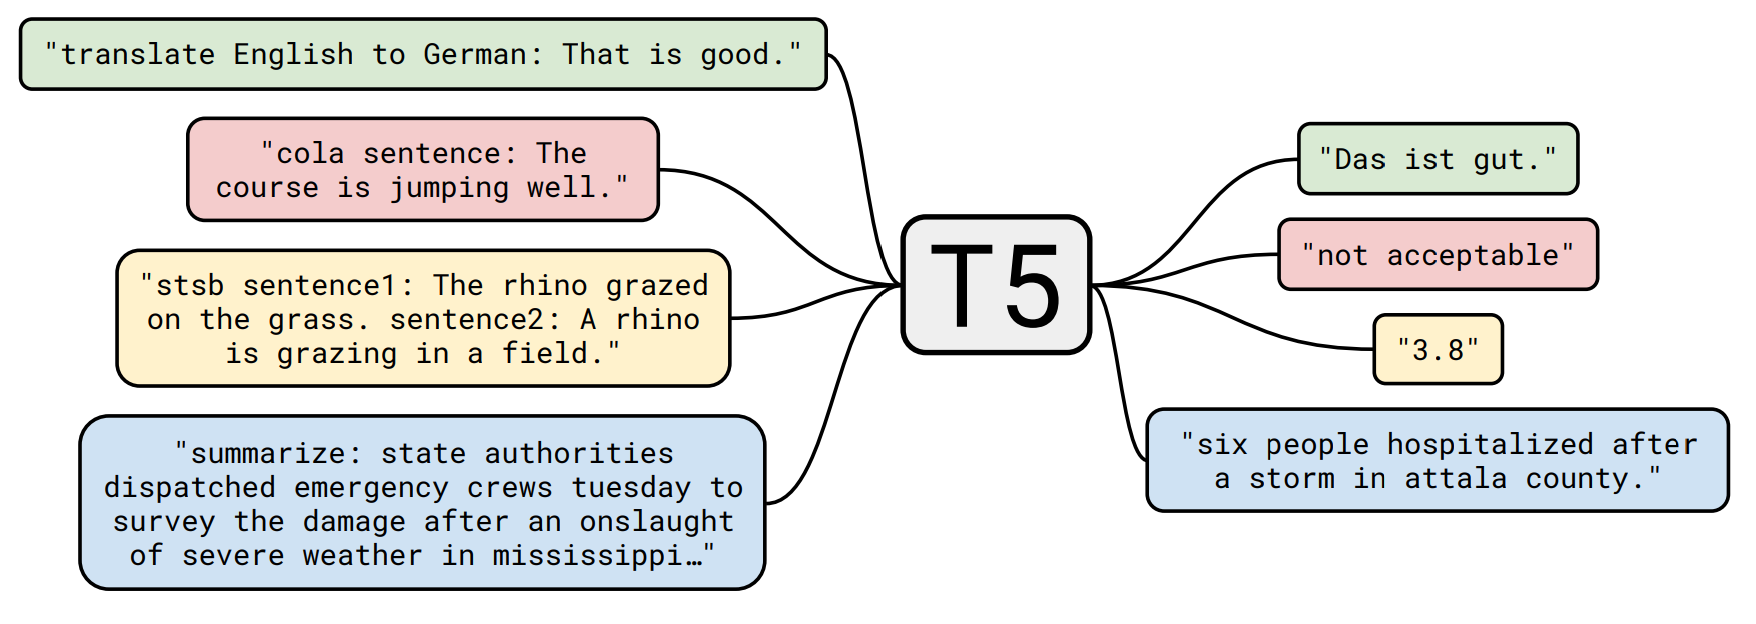
\includegraphics[width = 8cm]{figure/62-t5.png}\\ 
		\citebutton{Source: Raffel et al., 2020}{https://jmlr.org/papers/v21/20-074.html}
	\end{figure}

\pause

\begin{itemize}
    \item \ques The format used in T5 is not just any
    format, but it has a special property. Which property is this?

%\item A consistent format (as in T5) is desirable.


%How can we make the \textit{EXPLICIT}?
%    \item[$\to$] Mapping any natural language tasks into
%    a \textit{human-readable} prompted form
%\citebutton{Schick et al.,
%        2020}{https://arxiv.org/abs/2009.07118},
%\citebutton{Sanh et al., 2021}{https://arxiv.org/abs/2110.08207}
\end{itemize}

\vfill

\end{frame}




% ------------------------------------------------------------------------------

\begin{frame}{Carefully designing task formats (mostly prefixes)}

\vfill
	
	\begin{figure}
		\centering
		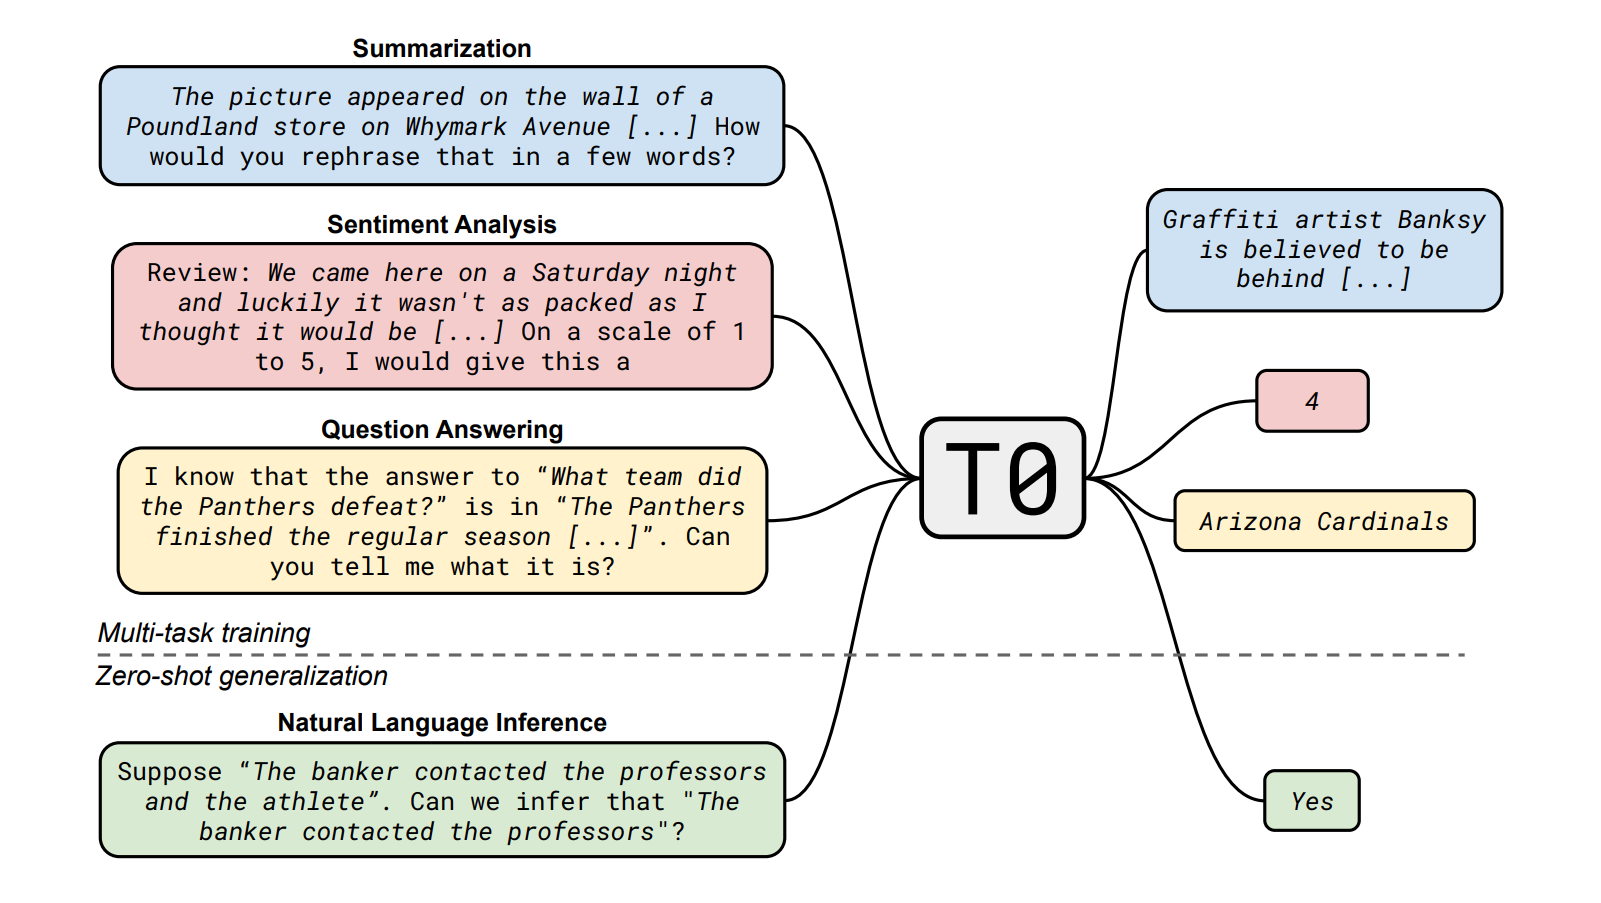
\includegraphics[width = 11cm]{figure/81-t0.png}\\ 
		\citebutton{Source: Sanh et al., 2021}{https://arxiv.org/abs/2110.08207}
	\end{figure}

\vfill

\end{frame}

% ------------------------------------------------------------------------------

\begin{frame}{T0 authors call this ``Multitask Prompted
		Training''}

\vfill

\begin{itemize}
    \item \textit{Multitask Prompted Training:} This
    training method involves learning from multiple
    tasks using unified prompt formats as a means to improve
    generalization to new, unseen tasks.
    \item This means that the model can perform well on tasks it hasn't been explicitly trained on.
    \item The key for this lies in the set of shared prompts it has learned from during fine-tuning.
\end{itemize}

\vfill

\end{frame}

% ------------------------------------------------------------------------------

\begin{frame}{Multitask Prompted Training}

\vfill

\begin{itemize}
    \item Benchmark for Evaluation:
        \begin{itemize}
        \item Instead of using held-out *samples* (as is
        standard in NLP) \ldots
        \item \ldots we now use held-out *tasks*
%            \item Held-out \textit{tasks} instead of just held-out samples as a test set\\
            \item All data sets belonging to a held-out task go to the test set
            \item Generalization across tasks %/ data distributions
        \end{itemize}
    \item Highlights the importance of prompts: The paper
        emphasizes the importance of prompts in facilitating
        transfer to new tasks, as the model can generalize to new tasks by relying on the learned prompts and the ability to generate text outputs.
\end{itemize}

\vfill

\end{frame}

% ------------------------------------------------------------------------------

\begin{frame}{T0: training and test tasks}

\vfill
	
	\begin{figure}
		\centering
		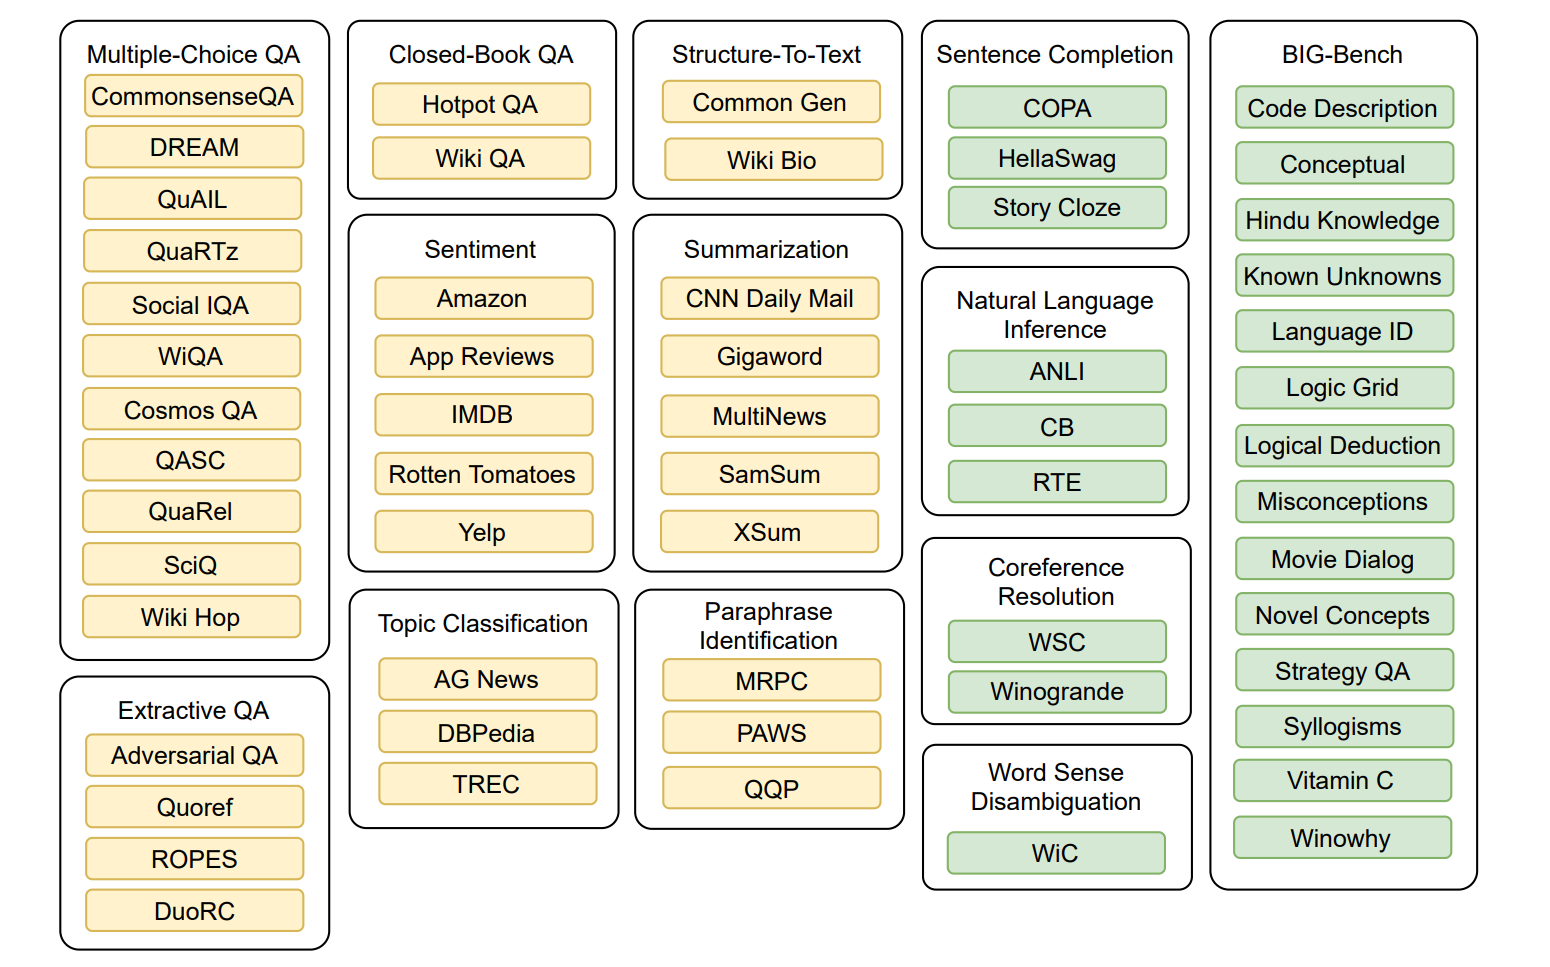
\includegraphics[width = 11cm]{figure/81-t0-data.png}\\ 
		\citebutton{Source: Sanh et al.,
		2021}{https://arxiv.org/abs/2110.08207} \ques
		What is an easy task? What is a hard task?
	\end{figure}

\vfill

\end{frame}

% ------------------------------------------------------------------------------

\begin{frame}{t0 -- prompt templates}

\vfill
	
	\begin{figure}
		\centering
		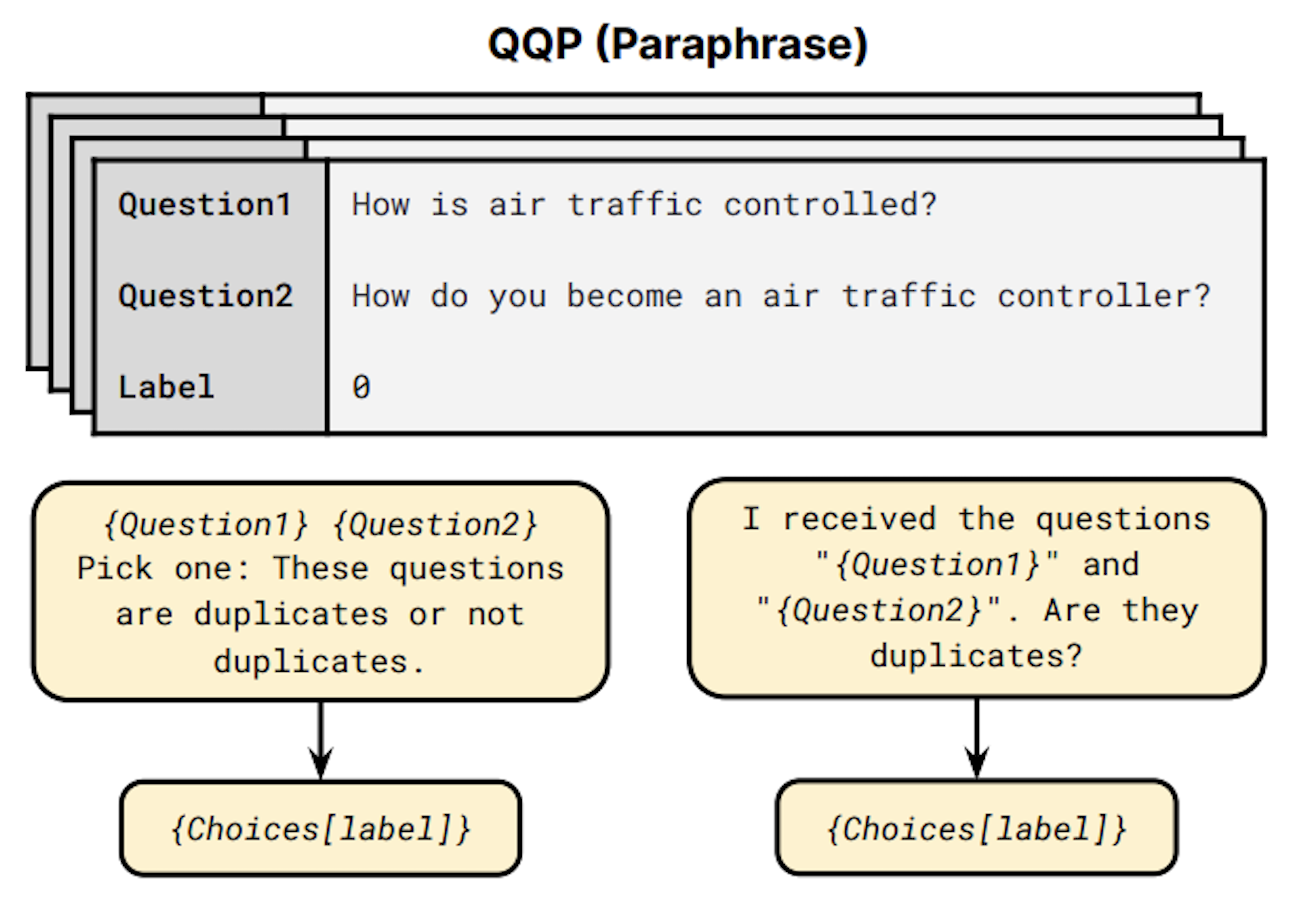
\includegraphics[height=7cm]{figure/t0ex1}\\ 
		\citebutton{Source: Sanh et al., 2021}{https://arxiv.org/abs/2110.08207}
	\end{figure}

\vfill

\end{frame}

\begin{frame}{t0 -- prompt templates}

\vfill
	
	\begin{figure}
		\centering
		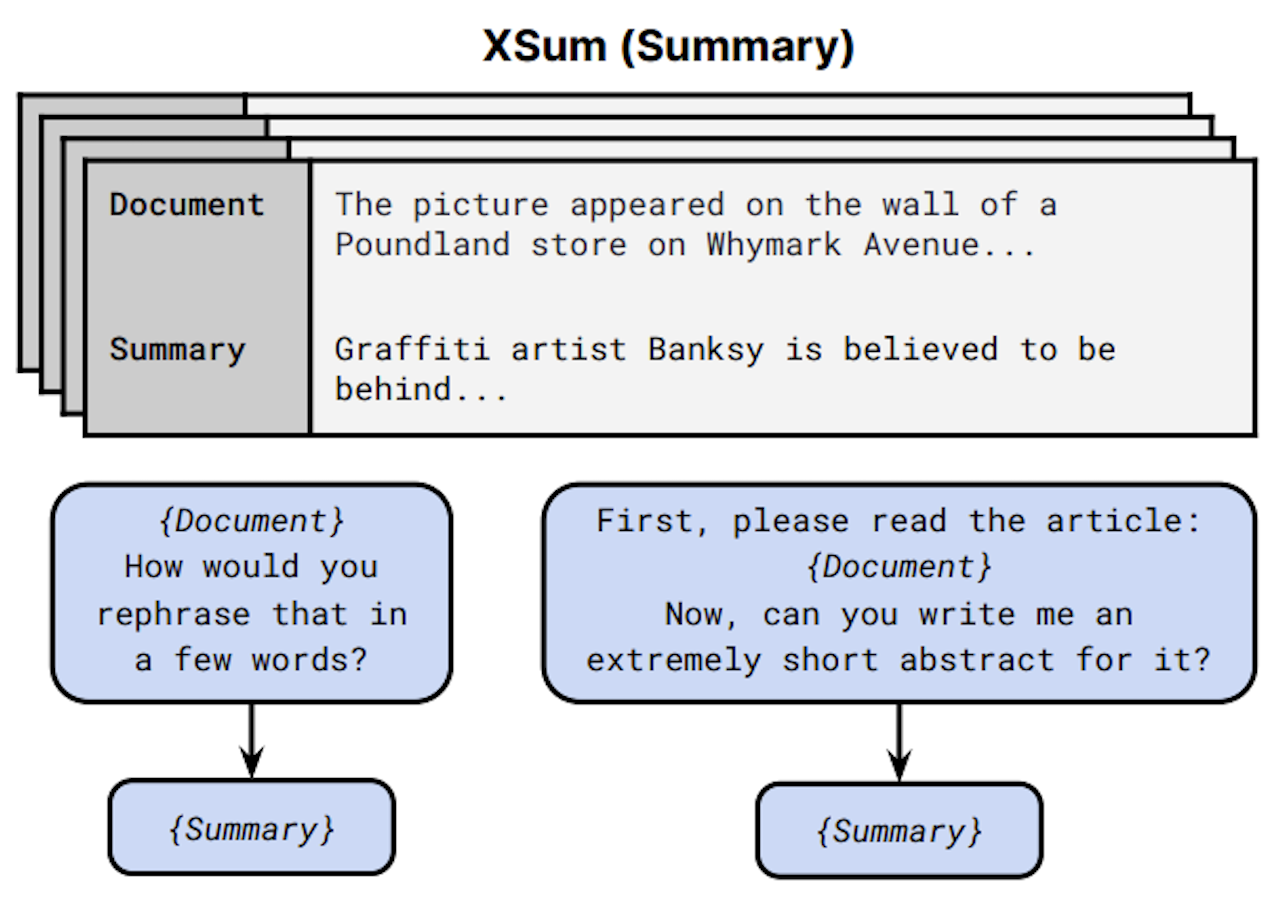
\includegraphics[height=7cm]{figure/t0ex2}\\ 
		\citebutton{Source: Sanh et al., 2021}{https://arxiv.org/abs/2110.08207}
	\end{figure}

\vfill

\end{frame}

% ------------------------------------------------------------------------------

\begin{frame}{finetuned language net (flan)}

\vfill
	
	\begin{figure}
		\centering
		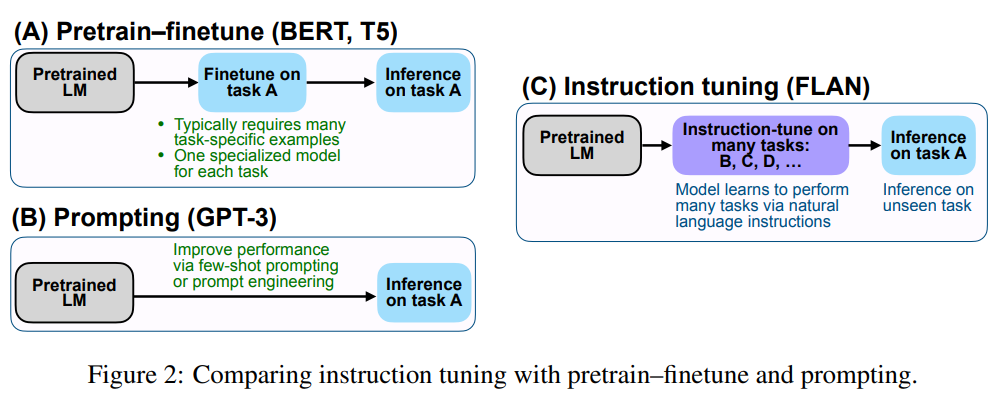
\includegraphics[width = 11cm]{figure/81-flan.png}\\ 
		\citebutton{Source: Wei et al., 2021}{https://arxiv.org/abs/2109.01652}
	\end{figure}

\vfill

\end{frame}

% ------------------------------------------------------------------------------

\begin{frame}{flan finetuning}

\vfill
	
	\begin{figure}
		\centering
		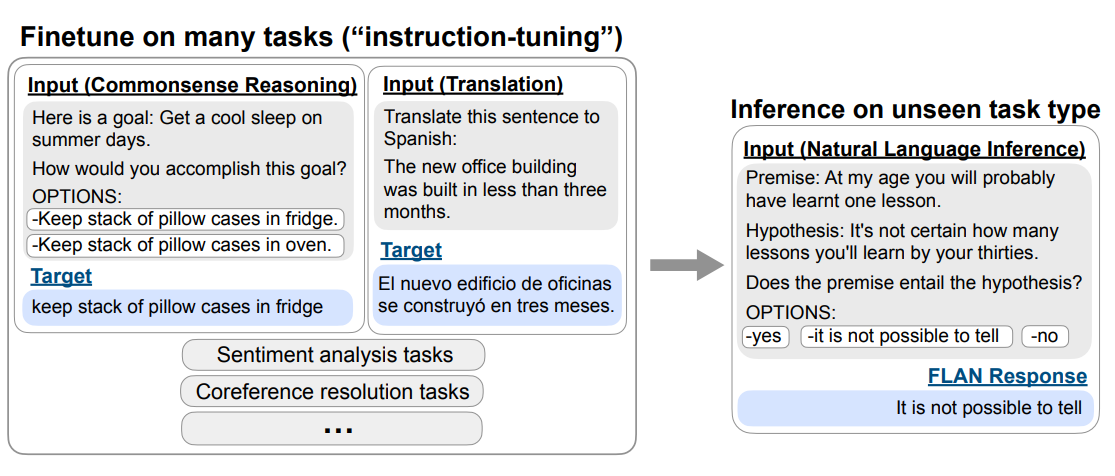
\includegraphics[width = 11cm]{figure/81-flan-instruct-tune.png}\\ 
		\citebutton{Source: Wei et al., 2021}{https://arxiv.org/abs/2109.01652}
	\end{figure}

\vfill

\end{frame}

% ------------------------------------------------------------------------------

\begin{frame}{flan performance}

\vfill
	
	\begin{figure}
		\centering
		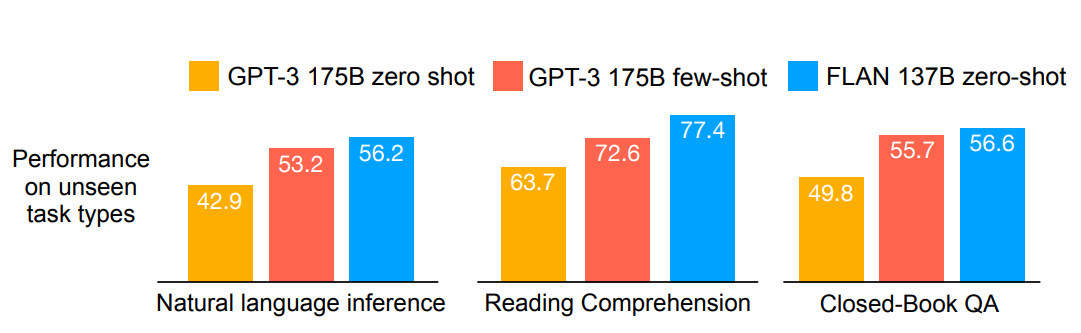
\includegraphics[width = 11cm]{figure/81-flan-perf.png}\\ 
		\citebutton{Source: Wei et al., 2021}{https://arxiv.org/abs/2109.01652}
	\end{figure}

\vfill

\end{frame}

% ------------------------------------------------------------------------------ 

\begin{vbframe}{Flan Fine-Tuning}

\vfill

\textbf{Extend multi-task learning} \vskip3mm

\begin{itemize}
\item Scaling the number of tasks and data
    \begin{itemize}
    \item NIV2 (1554 tasks)
    \item T0-SF (193 tasks)
    \item Muffin (80 tasks)
    \item CoT (reasoning tasks, cf. next chapter)
    \end{itemize}
\item Scaling model sizes
    \begin{itemize}
    \item PaLM 8\,B
    \item PaLM 62\,B
    \item PaLM 540\,B
    \end{itemize}
\end{itemize}

\vfill

\end{vbframe}

% ------------------------------------------------------------------------------ 

\begin{vbframe}{Flan upscaling}

\vfill

\textit{Fine-tuning in 1.8\,K tasks}
    
\begin{figure}
    \centering
    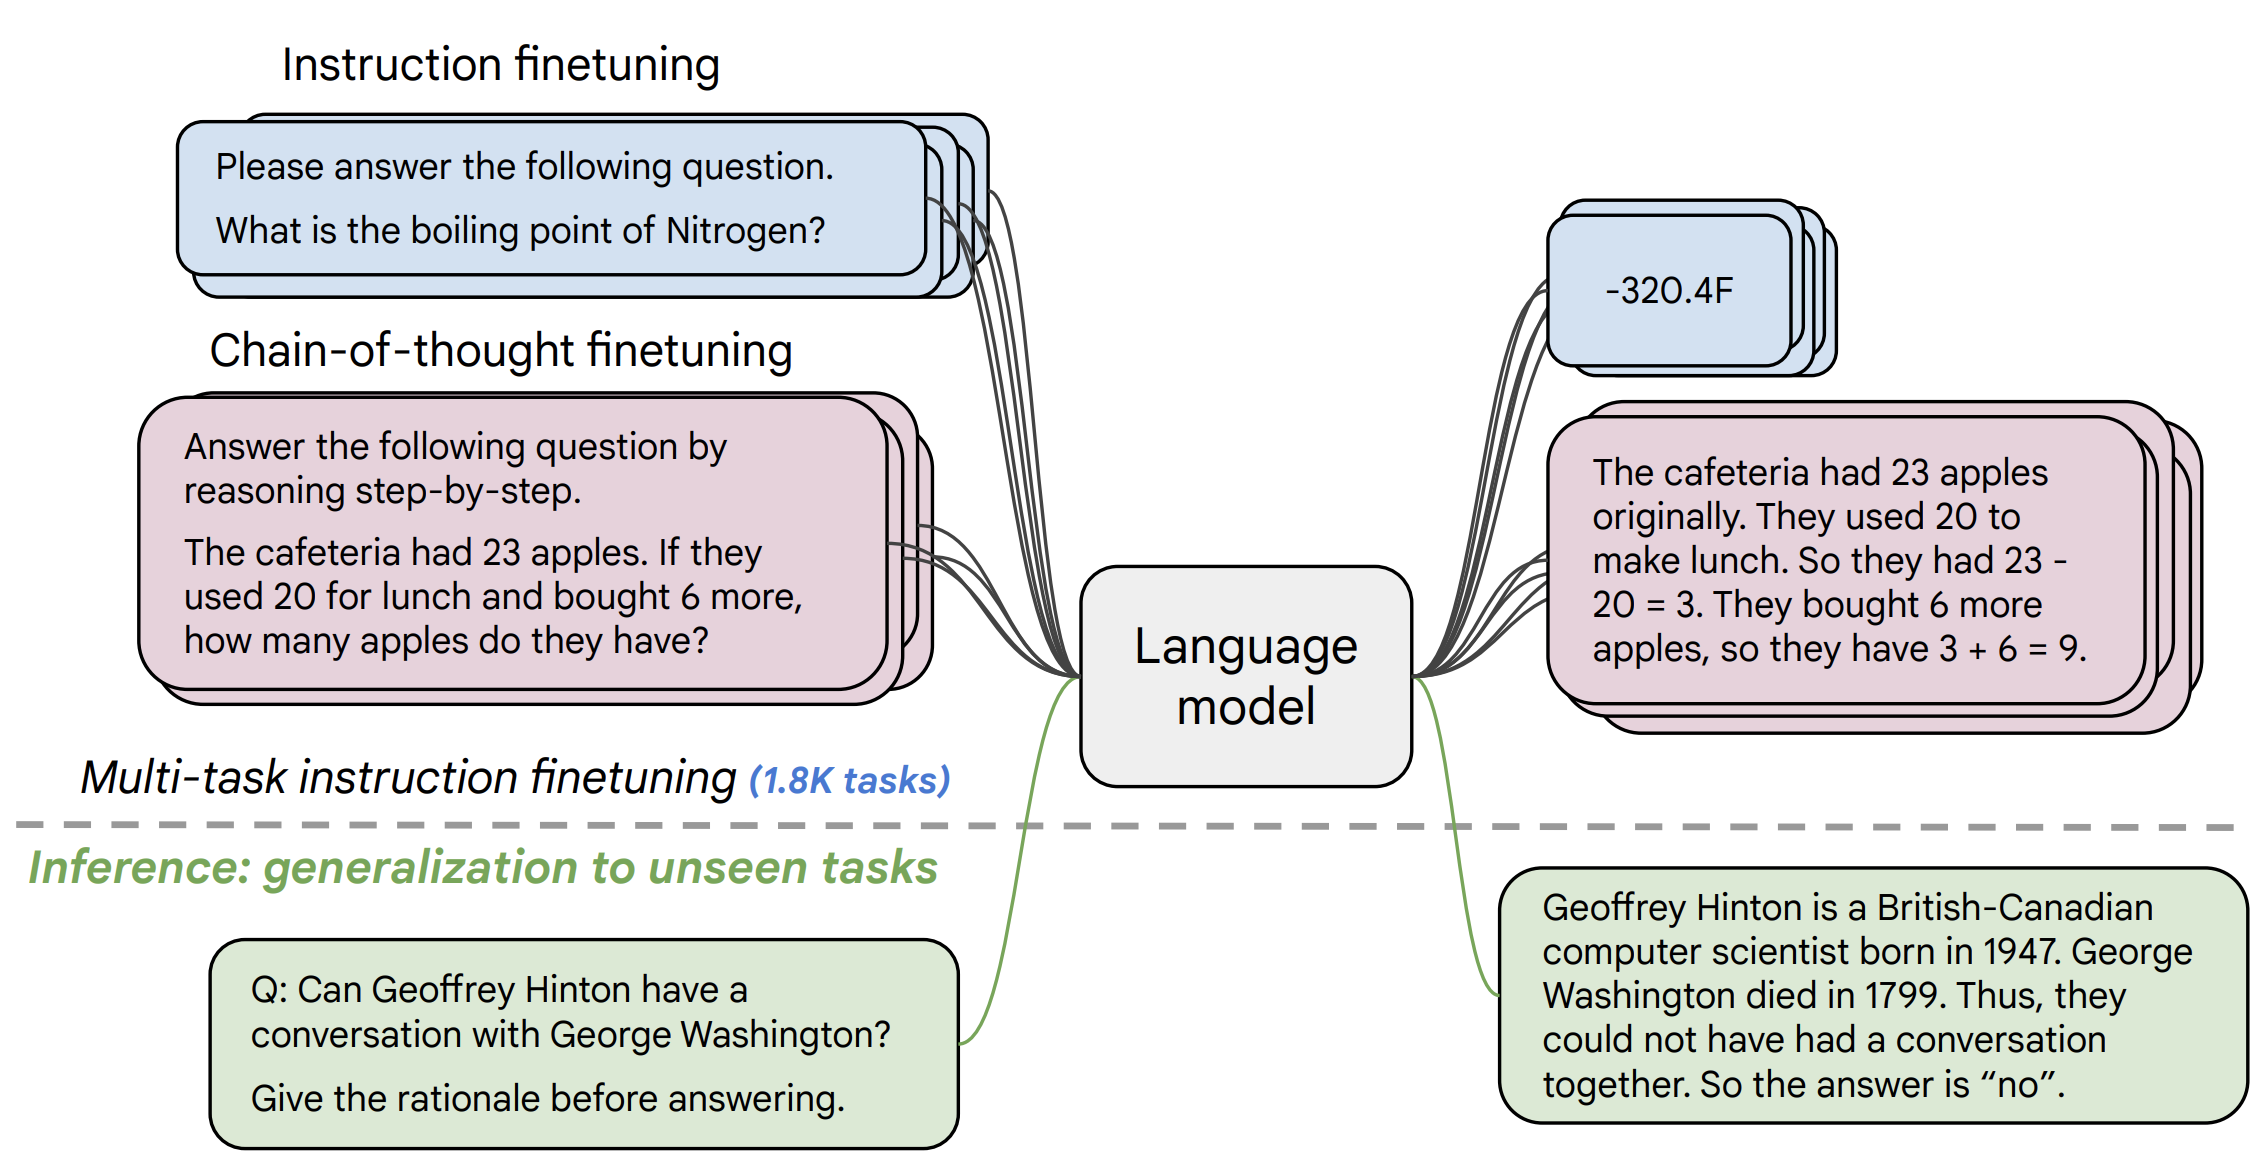
\includegraphics{figure/scaling_up_paradigms.png}\\
\citebutton{Source: Chung et al., 2022}{https://arxiv.org/pdf/2210.11416.pdf}
\end{figure}

\vfill

\end{vbframe}

% ------------------------------------------------------------------------------
\begin{vbframe}{Multi-task training vs Instruction tuning}

\vfill

\begin{itemize}
\item The term ``instruction tuning'' was introduced by FLAN paper,
		\citebutton{Source: Wei et al., 2021}{https://arxiv.org/abs/2109.01652}
\item However, today ``instruction tuning'' refers to a wide
variety of methods that train on instruction-output pairs,
    not just tasks
    \item
Open-ended generation and ``alignment'' 
is now included under
    the rubric ``instruction tuning'': brainstorming,
    writing a joke, give me ten analogies for concept X,
    don't use hate language, don't take positions on
    controversial political issues etc
\item These are not classical NLP tasks.
\item See next lecture
\item Our use of terminology in this class:
\item multi-task finetuning = tasks in the classical NLP
    sense
    \item instruction-tuning: a broad approach to changing
    the behavior of a raw language model (i.e., trained on
    next-word prediction) to be ``helpful, harmless and
    honest''. This includes training on classical NLP tasks,
    but it's just one part.
\end{itemize}

\vfill

\end{vbframe}
% ------------------------------------------------------------------------------

\begin{vbframe}{Fine-Tuning Conclusions}

\vfill

\begin{itemize}
\item The  more the better
    \begin{itemize}
    \item The more parameters the better
    \item The more training tasks the better
    \end{itemize}
\item Multi-task finetuning generalizes across models
    \begin{itemize}
    \item It works well on different architectures
    \end{itemize}
\item Greatly improves usability
%and mitigates some harms
\item It is relatively compute-efficient
    \begin{itemize}
    \item Pretraining is hugely expensive, finetuning and
    instruction tuning are usually much cheaper.
    \item For PaLM 540\,B it takes 0.2\,\% of pre-training compute, but improves by 9.4\,\%
    \end{itemize}
\end{itemize}

\vfill

\end{vbframe}



\begin{frame}{T0 vs Flan: Difference?}

\vfill
	
	\begin{figure}
		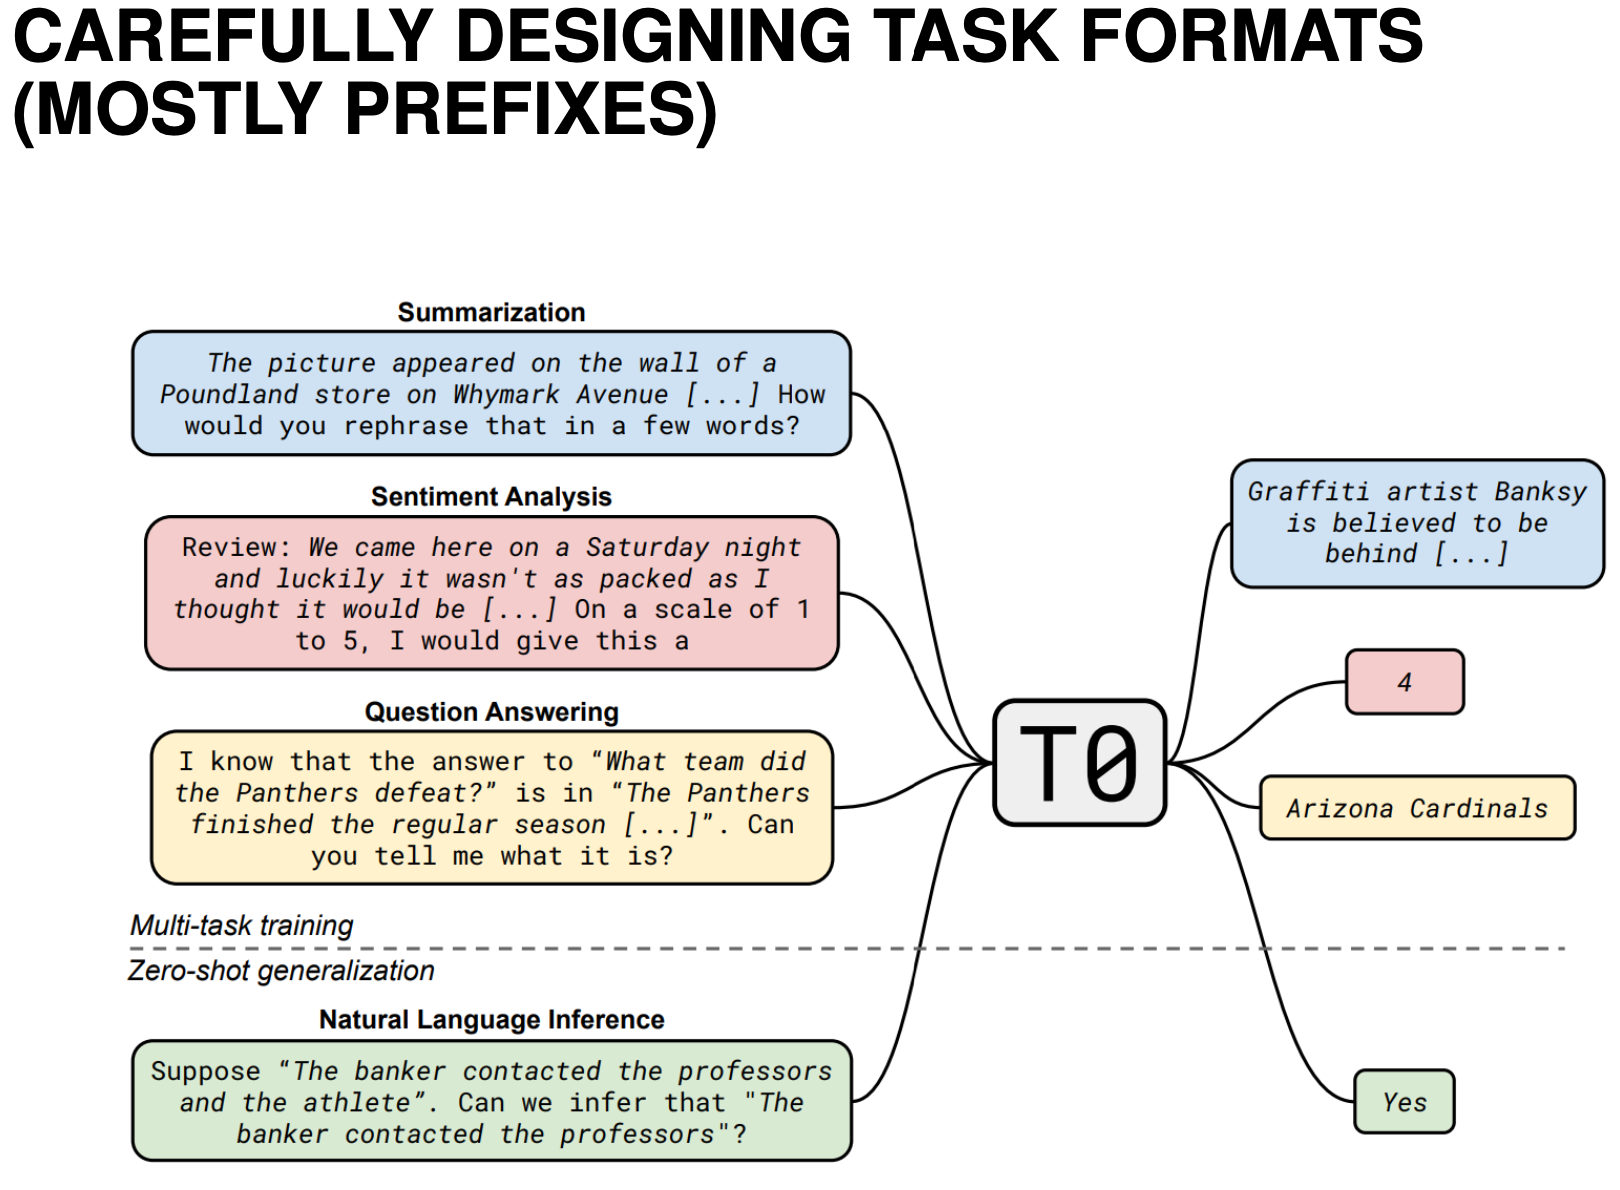
\includegraphics[width=5cm]{figure/t0comparison}
		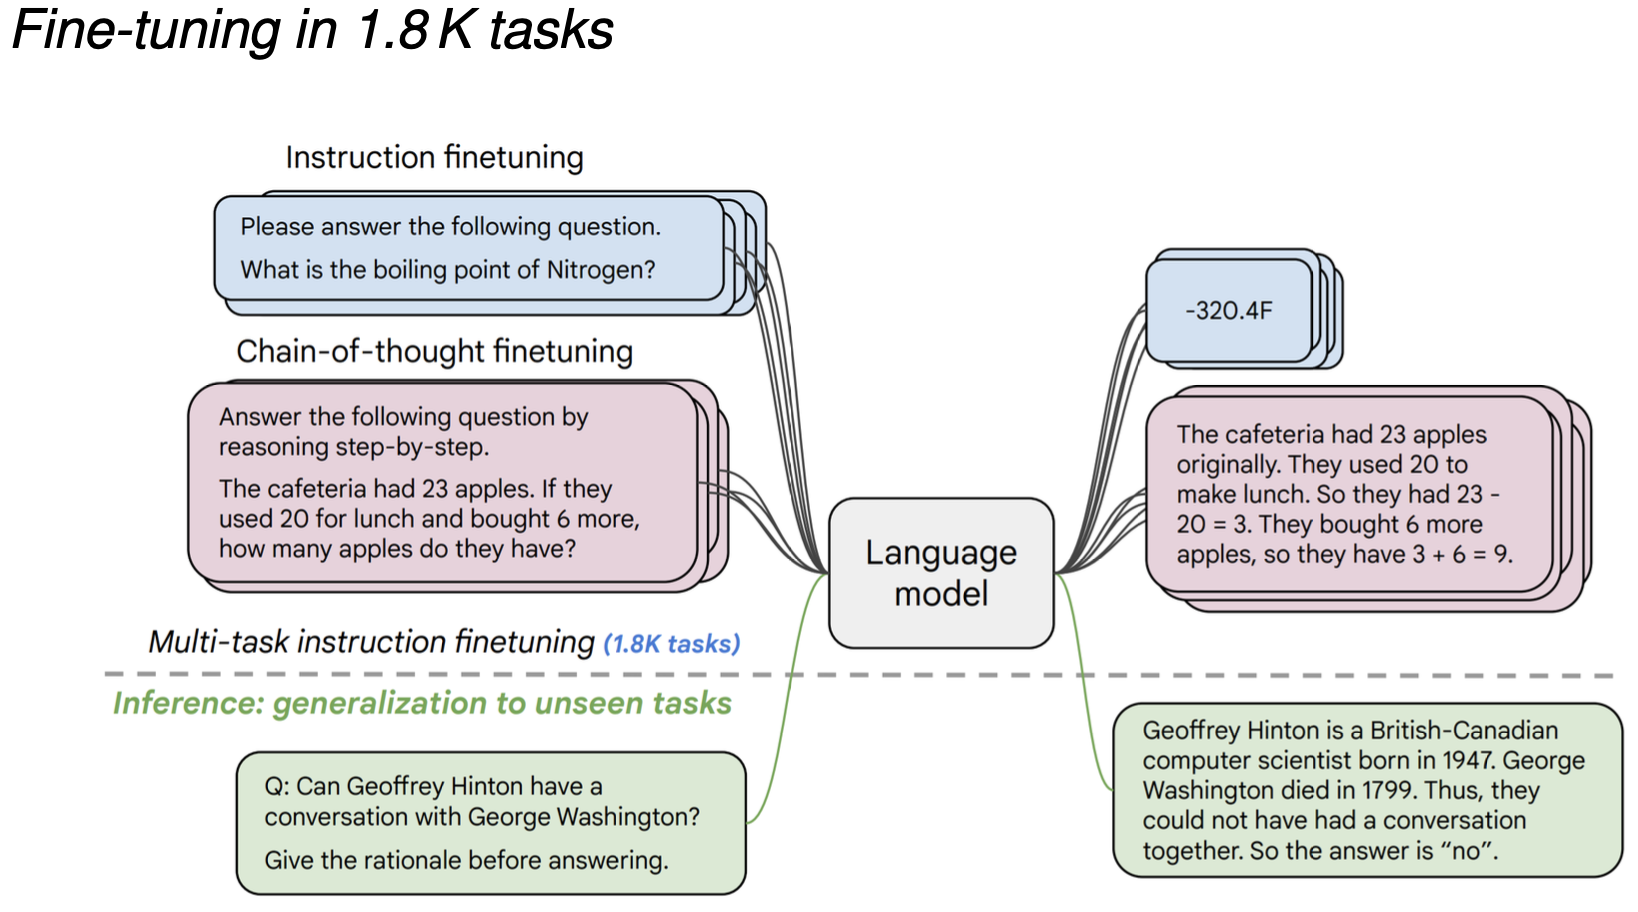
\includegraphics[width=5cm]{figure/flancomparison}
	\end{figure}

\vfill

\end{frame}


\endlecture
\end{document}




























% ------------------------------------------------------------------------------

\begin{vbframe}{Interactive NLP (\MakeLowercase{i}NLP)}

\vfill

\emph{\NoCaseChange{i}NLP considers language models as agens capable of observing, acting, and receiving feedback in a loop with external objets such as humants, knowledge bases, tools, models and environments.} \vskip2mm

\footnotesize{Source:} \href{https://arxiv.org/pdf/2305.13246.pdf}{\footnotesize \it Wang et al. (2023)}

\vfill

\end{vbframe}

% ------------------------------------------------------------------------------

\begin{vbframe}{Five levels of word scope}

\vfill

\begin{enumerate}

    \item Corpus
        \begin{itemize}
        \item Classical resource
        \end{itemize}

    \item Internet 
        \begin{itemize}
        \item Extra knowledge
        \end{itemize}

    \item Perception 
        \begin{itemize}
        \item multimodal LLMs
        \end{itemize}

    \item Embodiment 
        \begin{itemize}
        \item Interactive loops involving agents
        \end{itemize}

    \item Social 
        \begin{itemize}
        \item Interactive loops involving humans and environments
        \end{itemize}

\end{enumerate}

\vfill

\end{vbframe}

% ------------------------------------------------------------------------------

\begin{vbframe}{Supervised Instruction Tuning}

\vfill

Fine-tuning a PLM using data that provides task instruction supervision. \vskip3mm
\begin{itemize}
\item Supervised instructions on a multitask mixture
\item Instructions as part of input
\item Covering various tasks 
\item Enables transfer to unseen tasks, based on using a
common prompt template
\item Avoiding catastrophic forgetting
\end{itemize}

\vfill

\end{vbframe}

% ------------------------------------------------------------------------------

\begin{vbframe}{Continual Learning}

\vfill

\begin{itemize}
\item LLMs get outdated over time
\item It is beneficial to update them with new data
\item Continuously integrate knowledge from novel sources
\item Avoid catastrophic forgetting in various ways
    \begin{itemize}
    \item Regularization
    \item Rehearsal
    \item Modularization
    \end{itemize}
\end{itemize}

\vfill

\end{vbframe}

% ------------------------------------------------------------------------------

\begin{vbframe}{Parameter-Efficient Fine-Tuning}

\vfill

\begin{itemize}
\item Computationally hard to fine-tune very large models
\item Only update a small number of parameters
\item Two main categories:
    \begin{itemize}
    \item Partial fine-tuning updates only a strict subset of model parameters
    \item Adapter-based methods freeze the complet model and addess a small set of extra parameters which are tuned
    \end{itemize}
\end{itemize}

\vfill

\end{vbframe}

% ------------------------------------------------------------------------------

\begin{vbframe}{Semi-Supervised Fine-Tuning}

\vfill

\begin{itemize}
\item Use both labeled and unlabeled data to tune the model
\item Some of the interaction messages lack instructions
\item Other strategies:
    \begin{itemize}
    \item Self-training that uses model-generated data to tune the model itself
    \item Semi-supervised knowledge distillation that uses the model to annotate data for its tuning
    \end{itemize}
\end{itemize}

\vfill

\end{vbframe}

% ------------------------------------------------------------------------------
